\documentclass{article}
\usepackage{fullpage,palatino,mathpazo,amsmath,amssymb,url}
\usepackage{url,amsmath,amssymb,subfigure,boxedminipage,shadow}
\usepackage[pdftex]{graphicx,color}
\usepackage{hevea}
\graphicspath{{Figures/}}

\newcommand{\operator}{ \verb!Operator! }

\title{FloPoCo \input{../../VERSION} developer manual
}

\author{Florent de Dinechin, Bogdan Pasca}

\graphicspath{{Figures/}}
\pagestyle{empty}

\begin{document} 
\sloppy



\maketitle


Welcome to new developers! 

The purpose of this document is to help you design an operator within the
FloPoCo project.

 \section{Getting started with FloPoCo}


\subsection{Getting the source and compiling using CMake}

It is strongly advised that you work with the svn version of the
source, which can be obtained by following the instructions on
\url{https://gforge.inria.fr/scm/?group_id=1030}. If you wish to
distribute your work with FloPoCo, do not hesitate to contact us.

If you are unfamiliar with the CMake system, there is little to learn,
really. When adding .hpp and .cpp files to the project, you will need
to edit \texttt{CMakeLists.txt}. It is probably going to be straightforward,
just do some imitation of what is already there. Anyway \texttt{cmake} is well
documented. The web page of the CMake project is \url{http://www.cmake.org/}.


\subsection{Overview of the source code}

In FloPoCo, everything is an \texttt{Operator}. Operator is a virtual
class, all FloPoCo operators inherit this class. A good way to design
a new operator is to imitate a simple one. We suggest
%\texttt{IntAdder} or 
\texttt{Shifter} for simple integer operators, and \texttt{FPAdder}
for a complex operator with several sub-components. An example of
assembling several FP operators in a larger pipeline is
\texttt{Collision}.

 Meanwhile, browse
through \texttt{Operator.hpp}. It has become quite bloated, showing
the history of the project. Try not to use methods flagged as
deprecated, as they will be removed in the future.  Instead, use the
automatic pipeline framework is described in Section~\ref{sec:pme}
below.

Another important class hierarchy in FloPoCo is \texttt{Target}, which
defines the architecture of the target FPGA. It currently has two
sub-classes, \texttt{VirtexIV} and \texttt{StratixII}. You may want to
add a new target, the best way to do so is by imitation. Please
consider contributing it to the project.

To understand the command line, go read \texttt{main.cpp}. It is not
the part we are the most proud of, but it does the job.

The rest is arithmetic!

And do not hesitate to contact us: \texttt{Florent.de.Dinechin} or
\texttt{Bogdan.Pasca}, at \texttt{ens-lyon.fr}

\begin{center}
  \begin{latexonly}
  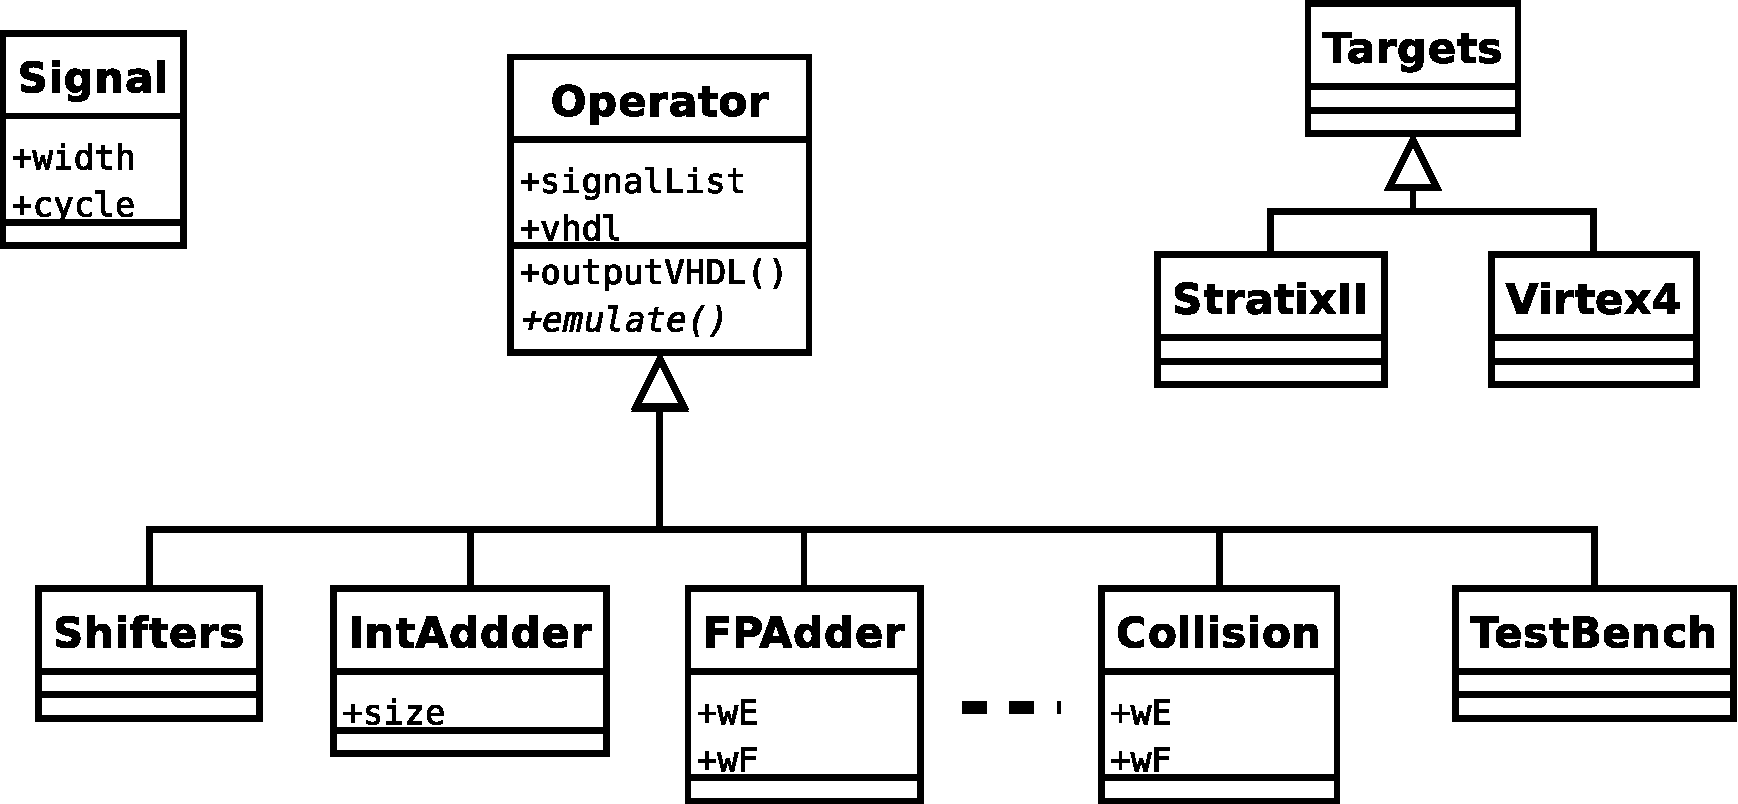
\includegraphics[width=0.7\textwidth]{../Figures/FloPoCoClasses.pdf}        
  \end{latexonly}
\end{center}

\section{Test bench generation}

The command\\
 \texttt{flopoco FPAdder 8 23 TestBench 500} \\
produces a test bench of 500 test vectors to exercise FPAdder.

\subsection{Operator emulation}


It requires only one additional method, \texttt{emulate}. As the name
indicates, this method provides a bit-accurate simulation of the operator. 
\begin{itemize}
\item Most operators should be fully specified: for a given input
  vector, they must output a uniquely defined vector. Imitate
  \texttt{IntAdder} for an integer operator. For floating-point
  operators, this unique output is the combination of a mathematical
  function and a well-defined rounding mode. The bit-exact MPFR
  library is used in this case. Imitate \texttt{FPAdder} in this case.

\item Other operators are not defined so strictly, and may take
  several output values. The last parameter of \texttt{addOutput}
  defines how many values this output may take. An acceptable
  requirement in floating-point is \texttt{faithful rounding}: the
  operator should return one of the two FP values surrounding the
  exact result. These values may be obtained thanks to the
  \emph{rounding up} and \emph{rounding down} modes supported by
  MPFR. See \texttt{FPLog} for a simple example, and
  \texttt{Collision} for a more complex example (computing the two
  faithful values for $x^2+y^2+z^2$).
\end{itemize}

\subsection{Operator-specific test  vector generation}
Overloading \texttt{\small emulate()} is enough for FloPoCo to be able
to create a generic test bench using random inputs. However, function
analysis also allows for better, more operator-specific test-case
generation. Let us just take two examples.

\begin{itemize}\item 
  A double-precision exponential returns $+\infty$ for all inputs
  larger than 710 and returns $0$ for all inputs smaller than
  $-746$. In other terms, the most interesting test domain for this
  function is when the input exponent is between $-10$ and $10$, a
  fraction of the full double-precision exponent domain ($-1024$ to
  $1023$). Generating random 64-bit integers and using them as
  floating-point inputs would mean testing mostly the
  overflow/underflow logic, which is a tiny part of the operator.


\item In a floating-point adder, if the difference between the exponents
  of the two operands is large, the adder will simply return the
  biggest of the two, and again this is the most probable situation
  when taking two random operands. Here it is better to generate
  random cases where the two operands have close exponents.
\end{itemize}
  Such cases are managed by overloading the Operator method
  \texttt{\small buildRandomTestCases()}. Finally,
  \texttt{\small buildStandardTestCases()} allows to test corner cases which
  random testing has little chance to find.


\section{Pipelining made easy: a tutorial}
\label{sec:pme}

Let us consider a toy MAC unit, which in VHDL would be written
\begin{verbatim}
library ieee;
use ieee.std_logic_1164.all;
use ieee.std_logic_arith.all;
use ieee.std_logic_unsigned.all;
library work;

entity MAC is
   port ( X   : in  std_logic_vector(63 downto 0);
          Y,Z : in  std_logic_vector(31 downto 0);
          R : out  std_logic_vector(63 downto 0)   );
end entity;

architecture arch of MAC is
  signal T: std_logic_vector(63 downto 0);
begin
   T <= Y * Z;
   R <= X + T;
end architecture;
\end{verbatim}
We chose for simplicity a fixed-size operator, but all the following
works as well for parameterized operators.

We have above  the description of
a combinatorial circuit. We now show how to turn it into a pipelined
one.


\subsection{First steps in FloPoCo}

FloPoCo mostly requires you to copy the part of the VHDL that is
between the \texttt{begin} and the \texttt{end} of the architecture
into the constructor of a class that inherits from
\verb!Operator!. The following is minimal FloPoCo code for
\verb!MAC.cpp!:
\begin{verbatim}
#include "Operator.hpp"

class MAC : public Operator
{
public:
// The constructor
MAC(Target* target): Operator(target)
{
	setName("MAC");
	setCopyrightString("ACME MAC Co, 2009");		

	// Set up the IO signals
	addInput ("X"  , 64);
	addInput ("Y"  , 32);
	addInput ("Z"  , 32);
	addOutput("R"  , 64);

   vhdl << declare("T", 64) << " <= Y * Z;" << endl;
   vhdl << "R <= X + T;" << endl;
}

// the destructor
	~MAC() {}
\end{verbatim}
 
And that's it. \verb!MAC! inherits from \verb!Operator! the method
\verb!outputVHDL()! that will assemble the information defined in the
constructor into synthesizable VHDL.

So far we have gained little, except that is is more convenient to
have the declaration of \verb!R! where its value is defined. Let us
now turn this design into a pipelined one.


\subsection{Basic pipeline}


Let us first insert a synchronization barrier between the result of the multiplication and the adder input. The code becomes: 

\begin{verbatim}
(...)
   vhdl << declare("T", 64) << " <= Y * Z;" << endl;
   nextCycle();
   vhdl << "R <= " << use("X") << " + " << use("T") << ";" << endl;
(...)
\end{verbatim}

Now this code will produce a properly synchronized pipelined operator
with \verb!-pipeline=yes!, and will produce a combinatorial operator
(the same as previously) with \verb!-pipeline=no!.

How does it work? 
\begin{itemize}\item 
  \verb!Operator! has a \verb!currentCycle! attribute, initially equal to
  zero. The main function of 	\verb!nextCycle()! is to increment \verb!currentCycle!.

\item Every signal declared through \verb!addInput! or \verb!declare!
  has a \verb!cycle! attribute, which represents the cycle at which
  this signal is active. It is 0 for the inputs, and for signals
  declared through \verb!declare()! it is \verb!currentCycle!  at the
  time \verb!declare! was invoked.

\item Every signal also possesses an attribute \verb!lifeSpan! which
  indicates how many cycles it will need to be delayed. This attribute
  is initialized to 0, then possibly increased by \verb!use()! as we
  will see below. When the \verb!lifeSpan! of a signal \verb!X!  is
  greater than zero, \verb!outputVHDL()! will create \verb!lifeSpan!
  new signals \verb!X_d1!, \verb!X_d2! and so on, and insert registers
  between them. In other words, \verb!X_d2! will hold the value of
  \verb!X! delayed by 2 cycles.

\item Wrapping a signal in \verb!use()! has the following  effect. First,
  \verb!use("X")! will compare \verb!currentCycle! and the
  \verb!cycle! declared for \verb!X!, which we note \verb!X.cycle!. 
  \begin{itemize}\item 
    If they are equal, or if \verb!-pipeline=no!, \verb!use("X")! will
    simply return \verb!"X"!.
  \item If \verb!currentCycle! $<$ \verb!X.cycle!, \verb!use("X")!
    will emit an error message complaining that \verb!X! is being
    used before the cycle at which it is defined.
  \item If \verb!currentCycle! $>$ \verb!X.cycle!, \verb!use("X")!
    will delay signal \verb!X! by
    n=\verb!currentCycle!$-$\verb!X.cycle! cycles. Technically
    \verb!use("X")! just returns \verb!"X_dn"!, and updates \verb!X.lifeSpan! to be at least equal to n.
  \end{itemize}
\end{itemize}

It should be noted that this scheme gracefully degrades to a
combinatorial operator. It also automatically adapts to random
insertions and suppressions of synchronization barriers. Typically,
one synthesizes an operator, and decides to break the critical path by
inserting a synchronisation barrier in it. This may be as simple as
inserting a single \verb!nextCycle()! in the code. FloPoCo takes care of the rest.

It is also possible to have \verb!if!s before some of the
\verb!nextCycle()!, so that the pipeline adapts to the frequency, the
operator generic parameters, etc. See \verb!IntAdder! for an example.

Some more notes:
\begin{itemize}
\item The second parameter of \verb!declare()!, the signal width, is
  optional and defaults to 1 (a \verb!std_logic! signal).

\item Other functions allow to manipulate \verb!currentCycle!. They
  are \verb!setCycle(int n)!, \verb!setCycleFromSignal(string s)!
  which sets the \verb!currentCycle! to the \verb!cycle! of the
  signal whose name is given as an argument (going back if needed),
  and \verb!syncCycleFromSignal(string s)! which may only advance \verb!currentCycle!. The latter allows to synchronise
  several signals by setting \verb!currentCycle! to the max of their
  \verb!cycle!. See \verb!FPAdder! or \verb!FPLog! for examples of
  such synchronisations. 

All these functions have an optional boolean
  second argument which, if true, inserts in the generated VHDL a
  comment ``-- entering cycle n''.


\item If our toy example, is part of a larger circuit such that X is
  itself delayed, the pipeline will adapt to that.

\end{itemize}

\subsection{Advanced pipeline with sub-components}

We now show how to replace the + and * with FloPoCo pipelined
operators. These operators support frequency-directed pipelining,
which means that the resulting MAC will also have its pipeline depth
automatically computed from the user-supplied frequency.

\begin{verbatim}
(...)
   // vhdl << declare("T", 64) << " <= Y * Z;" << endl;

	IntMultiplier my_mult = new IntMultiplier(target, 32, 32);
	oplist.push_back(my_mult); // some day this will be an addOperator method
	inPortMap   (my_mult, "X", "Y"); // formal, actual
	inPortMap   (my_mult, "Y", "Z");
	outPortMap  (my_mult, "R","T");
	vhdl << instance(my_mult, "my_mult"); // 2nd param is the VHDL instance name
   // advance to the cycle of the result
	syncCycleFromSignal("T"); 

   // pipelined operators do not have a register on the output 
   nextCycle();

   // vhdl << "R <= " << use("X") << " + " << use("T") << ";" << endl;

	IntAdder my_adder = new IntAdder(target, 64);
	oplist.push_back(my_adder);
	inPortMap   (my_adder, "X", "X");
	inPortMap   (my_adder, "Y", "T");
	inPortMapCst(my_adder, "Cin", "0"); -- carry in
	outPortMap  (my_adder, "R","RR");
	vhdl << instance(my_adder, "my_add");
   // advance to the cycle of the result
	syncCycleFromSignal("RR"); 
   vhdl << "R <= RR;" << endl; // no need for use since we are in the same cycle
(...)
\end{verbatim}


And that's it. In the code above, an \verb!inPortMap()! does the same
job as a \verb!use()!, and an \verb!outPortMap()! does the same job as
a \verb!declare()!, although it doesn't need a signal width since it
can read it from the sub-component. \verb!instance()! also has the
effect that \verb!outputVHDL()! will declare this component in the
VHDL header of \verb!MAC!.

\end{document}
